%-----------------------------------------------------------------------------------
%	PACKAGES AND OTHER DOCUMENT CONFIGURATIONS
%----------------------------------------------------------------------------------

\documentclass[11pt]{article}

\usepackage[top=2cm, bottom=3cm, left=2cm, right=2cm]{geometry}

\setlength{\parindent}{0in}

\newcommand{\Var}{\mathrm{Var}}

\newcommand{\Cov}{\mathrm{Cov}}

\newcommand{\plim}{\rightarrow_{p}}

\usepackage{amsmath, amsfonts}
\usepackage{graphicx}
\usepackage{pdfpages}
\usepackage{bm}
\usepackage{listings}
\usepackage{multirow,array}
\usepackage{enumerate}
\usepackage{bbm}


\usepackage[latin1]{inputenc}

\usepackage{amssymb}

\usepackage{mathrsfs}
\usepackage{float}
\usepackage{booktabs}
\usepackage{color}
\usepackage{rotating}
\usepackage{amsthm}
\usepackage{multirow,array}
\usepackage{caption}
\usepackage{url}


\DeclareMathOperator*{\argmax}{arg\,max}
\DeclareMathOperator*{\argmin}{arg\,min}



% Expectation symbol
\newcommand{\E}{\mathrm{E}}
\newcommand{\V}{\mathrm{V}}
\newcommand{\N}{\mathcal{N}}
\newcommand{\R}{\mathbb{R}} 

%----------------------------------------------------------------------------------
%	TITLE AND AUTHOR(S)
%----------------------------------------------------------------------------------
\title{Econ 675 Assignment 3} % The article title


\author{Nathan Mather\thanks{Shouts out to Ani for the help with question 1 }}  % The article author(s) 

\date{\today} % An optional date to appear under the author(s)


%----------------------------------------------------------------------------------
\begin{document}
	
%------------------------------------------------------------------------------
%	TABLE OF CONTENTS & LISTS OF FIGURES AND TABLES
%------------------------------------------------------------------------------
\maketitle % Print the title/author/date block

\setcounter{tocdepth}{2} % Set the depth of the table of contents to show sections and subsections only

\tableofcontents % Print the table of contents


%-------------------------------------------------------------
% Question 1 
%-------------------------------------------------------------

\section{Question 1: Many Instruments Asymptotics}

\subsection{Q1 Part 1}
The first two results follow immediately while the third follows from $ \E[x'u/n] = \E[v'u/n] = \sigma_{uv}$ since Z is non-random. for the ourth result, note that $\E[x'Pu]=\E[v'Pu]=k\sigma_{uv}$ because $\E[v_iu_j] = 0$ for all $i \neq j$ and $\sum_{i=1}^{n}P_{ij} = K$. Finally the last result follows analogously. 

\subsection{q1 Part 2}

$$ x'x/n = v'v/n + 2v'Z\pi/n + \pi'Z'Z\pi /n \plim \mu + \sigma_v^2$$

using LLN and because $\E[v'Z \pi/n ] =0 $ and $\V[v'Z\pi/n] = O(n^{-1}).$ which gives the first result. 

For the second result, note that 

$$x'Px/n = v'pv/n + 2v'Z\pi/n + \pi'Z'Z\pi/n \plim \mu + \rho \sigma_v^2$$

which follows from $E[v'Pv/n] = \sum_{i=1}^{n}p_{ii} \sigma_v^2/n = K\sigma_v^2 /n \rightarrow \rho\sigma_v^2$ , because $\E[v_iv_j] = 0$ for all $i\neq j$, and because $\V[v'pv/n] \rightarrow 0$ after some calculations and using basic projection matrices. Specifically, 

$$ \V[v'Pv/n] = \frac{1}{n^2} \V \left[ \sum_{i=1}^{n}p_{ii}v_i^2 + 2\sum_{i<j}^{} p_{ij} v_i v_j  \right] = \frac{1}{n^2} \left( \V[v_i^4] \sum_{i=1}^{n} p_{ii}^2 + 4\sigma_v^2 \sum_{i<j}^{}p^2_{ij} \right) \le \frac{C}{n^2} trace(P'P) \le \frac{CK}{n^2} \rightarrow 0
$$

Where C is some universal constant greater than zero. \\ \\ 

For the third result,

$$ x'Pu/n = \pi'Z'u/n + v'Pu/n \plim 0 + \rho \sigma_{uv}$$
which follows from a similar argument to the second result and part 1. 

\subsection{Q1 part 3 }

This follows directly by previous results because 

$$ \hat{\beta}_{2sls} = \beta + (x'Px/n)^{-1}x'Pu/n$$

and the result follows by CMT. 

\subsection{Q1 Part 4}

$$ \tilde{\beta_{2sls - BC}} = \beta + (x'Px)^{-1}(x'Pu - v'Pu) = \beta + (x'Px)^{-1}\pi'Z'u$$

By the argument to part 2, the second term is $o_p(1)$

\subsection{Q1 part 5}

(a) 
\begin{align*}
\bm{x}'\check{\bm{P}}\bm{u} &=(\bm{\pi}'\bm{Z}'+\bm{v}')(\bm{P} - \frac{K}{n}\bm{I}_n)\bm{u}\\
&=\bm{\pi}'\bm{Z}'(\bm{P} - \frac{K}{n}\bm{I}_n)\bm{u} + \bm{v}'(\bm{P} - \frac{K}{n}\bm{I}_n)\bm{u}\\
&=\bm{\pi}'\bm{Z}'(\bm{P} - \frac{K}{n}\bm{I}_n)\bm{u} + \left(\check{\bm{v}}' + \frac{\sigma^2_{uv}}{\sigma^2_u}\bm{u}'\right)(\bm{P} - \frac{K}{n}\bm{I}_n)\bm{u}\\
&=\bm{\pi}'\bm{Z}'(\bm{P} - \frac{K}{n}\bm{I}_n)\bm{u} + \check{\bm{v}}'(\bm{P} - \frac{K}{n}\bm{I}_n)\bm{u} + \frac{\sigma^2_{uv}}{\sigma^2_u}\bm{u}'(\bm{P} - \frac{K}{n}\bm{I}_n)\bm{u},
\end{align*}
as required.

(b)
Next, note that
\begin{align*}
\E[\bm{\pi}'\bm{Z}'(\bm{P} - \frac{K}{n}\bm{I}_n)\bm{u}] &= \bm{\pi}'\bm{Z}'\E[\bm{u}] - \frac{K}{n}\bm{\pi}'\bm{Z}'\E[\bm{u}] = 0,
\end{align*}
since $\bm{Z}$ is nonrandom. Accordingly, the CLT implies that
\begin{align*}
\frac{1}{\sqrt{n}} \bm{\pi}'\bm{Z}'(\bm{P} - \frac{K}{n}\bm{I}_n)\bm{u} \to_d \N(0, V_1(\rho)),
\end{align*}
where
\begin{align*}
V_1(\rho) &= \lim_{n\to \infty} \V[1/\sqrt{n}\bm{\pi}'\bm{Z}'(\bm{P} - \frac{K}{n}\bm{I}_n)\bm{u}]\\
&=\lim_{n\to \infty} \frac{1}{n}\E[\bm{\pi}'\bm{Z}'(\bm{P} - \frac{K}{n}\bm{I}_n)\bm{u}\bm{u}' (\bm{P} - \frac{K}{n}\bm{I}_n)\bm{Z}\bm{\pi}]\\
&=\lim_{n\to \infty} \frac{1}{n} \sigma^2_u \left[ \bm{\pi}'\bm{Z}'(\bm{P} - \frac{K}{n}\bm{I}_n)(\bm{P} - \frac{K}{n}\bm{I}_n)\bm{Z}\bm{\pi}\right]\\
&=\lim_{n\to \infty} \frac{1}{n} \sigma^2_u \left[ \bm{\pi}'\bm{Z}'\bm{Z}\bm{\pi}- 2\frac{K}{n}\bm{\pi}'\bm{Z}'\bm{Z}\bm{\pi} + \frac{K^2}{n^2}\bm{Z}\bm{\pi}'\bm{Z}'\bm{Z}\bm{\pi}\right]\\
&= \sigma^2_u (1-\rho^2).
\end{align*}

(c)
Now,
\begin{align*}
\E[ \check{\bm{v}}'(\bm{P} -K/n\bm{I}_n) \bm{u}] &= \E\left[\left({\bm{v}}' - \frac{\sigma^2_{uv}}{\sigma^2_u}\bm{u}'\right)\bm{P}\bm{u} - \frac{K}{n} \left({\bm{v}}' - \frac{\sigma^2_{uv}}{\sigma^2_u}\bm{u}'\right)\bm{u}\right]\\
&=\E[{\bm{v}}'\bm{P}\bm{u}] - \frac{\sigma^2_{uv}}{\sigma^2_u}\E[\bm{u}'\bm{P}\bm{u}] - \frac{K}{n}\E[\bm{v}'\bm{u}] + \frac{K}{n}\frac{\sigma^2_{uv}}{\sigma^2_u}\E[\bm{u}'\bm{u}]
\end{align*}
Then, plugging in the results from part 1 gives
\begin{align*}
\E[ \check{\bm{v}}'(\bm{P} -K/n\bm{I}_n) \bm{u}] &= K\sigma^2_{uv} - \frac{\sigma^2_{uv}}{\sigma^2_u} K \sigma^2_u - \frac{K}{n} \cdot n \sigma^2_{uv} + \frac{K}{n}\frac{\sigma^2_{uv}}{\sigma^2_u} \cdot n \sigma^2_u = 0,
\end{align*}
as required. \\

To get the convergence result we would do the following. Compute $\V[\check{\bm{v}}'(\bm{P} -K/n\bm{I}_n) \bm{u}]$. Using the assumption $\V[\bm{u}|\check{\bm{v}}] = \sigma^2_u\bm{I}_n$, it can be shown that
\begin{align*}
\lim_{n\to \infty} \V[\check{\bm{v}}'(\bm{P} -K/n\bm{I}_n) \bm{u}] = O(K).
\end{align*}
Then, we can somehow use the Markov inequality to get the desired convergence result.

\iffalse
Now, to show the convergence result note that
\begin{align*}
\check{\bm{v}}'(\bm{P} -K/n\bm{I}_n) \bm{u} &= {\bm{v}}'\bm{P}\bm{u} -  \frac{\sigma^2_{uv}}{\sigma^2_u}\bm{u}'\bm{P}\bm{u} - \frac{K}{n}\bm{v}'\bm{u} + \frac{K}{n}\frac{\sigma^2_{uv}}{\sigma^2_u}\bm{u}'\bm{u}
\end{align*}
Thus
\begin{align*}
\frac{1}{\sqrt{K}} \check{\bm{v}}'(\bm{P} -K/n\bm{I}_n) \bm{u} =  {\bm{v}}'\bm{P}\bm{u} -  \frac{\sigma^2_{uv}}{\sigma^2_u}\bm{u}'\bm{P}\bm{u} - \frac{K}{n}\bm{v}'\bm{u} + \frac{K}{n}\frac{\sigma^2_{uv}}{\sigma^2_u}\bm{u}'\bm{u}
\end{align*}
\fi

(d)
Analogous derivations to the above question give the desired results.

(e)
Now,
\begin{align*}
\E[\bm{x}'\check{\bm{P}}\bm{u}] &= \E[(\bm{\pi}'\bm{Z}'+\bm{v}')(\bm{P} -K/n\bm{I}_n)\bm{u}]\\
&= \E[\bm{\pi}'\bm{Z}'(\bm{P} -K/n\bm{I}_n)\bm{u}] + \E[\bm{v}'(\bm{P} -K/n\bm{I}_n)\bm{u}]\\
&=0 + \E[\bm{v}'\bm{P}\bm{u}] - K/n\E[\bm{v}'\bm{u}]\\
&= K \sigma^2_{uv} - K/n \cdot n \sigma^2_{uv}\\
&=0.
\end{align*}
And
\begin{align*}
\vartheta^2 = \V[\bm{x}'\check{\bm{P}}\bm{u}/\sqrt{n}] &= \frac{1}{n}\E[\bm{x}'\check{\bm{P}}\bm{u}\bm{u}'\check{\bm{P}}\bm{x}]\\
&=\frac{1}{n}\E[\bm{x}'(\bm{P} -K/n\bm{I}_n)\bm{u}\bm{u}'(\bm{P} -K/n\bm{I}_n)\bm{x}]\\
&=\frac{1}{n}\E[(\bm{x}'\bm{P}\bm{u} - K/n\bm{x}'\bm{u})(\bm{u}'\bm{P}\bm{x}-K/n\bm{u}'\bm{x})]
\end{align*}

(f)
Note that
\begin{align*}
\sqrt{n}(\hat\beta_{\texttt{2SLS}} - \beta) &= (\bm{x}'\check{\bm{P}}\bm{x}/n)^{-1}(\frac{1}{\sqrt{n}}\bm{x}'\check{\bm{P}}\bm{u})
\end{align*}
And we assume that
\begin{align*}
\frac{1}{\sqrt{n}}\bm{x}'\check{\bm{P}}\bm{u} \to_d \N(0, \vartheta^2)
\end{align*}
Thus,
\begin{align*}
\sqrt{n}(\hat\beta_{\texttt{2SLS}} - \beta) \to_d \N(0, \E[\bm{x}'\check{\bm{P}}\bm{x}]^{-1}\vartheta^2\E[\bm{x}'\check{\bm{P}}\bm{x}]^{-1})
\end{align*}











%-------------------------------------------------------------
% Question 2
%-------------------------------------------------------------

\section{Question 2: Weak Instruments Simulations}

\begin{center}
	
	\centering
	
	\textbf{Results for $n \gamma^2$ = 0}\par\medskip
	\scalebox{1}{
		% latex table generated in R 3.5.1 by xtable 1.8-3 package
% Tue Nov 13 14:50:16 2018
\begin{tabular}{llrrrrr}
  \hline
reg\_type & variable & mean & st.dev & quant .1 & quant .5 & quant .9 \\ 
  \hline
ols & estimate & 1.00 & 0.01 & 0.99 & 1.00 & 1.01 \\ 
  ols & std.error & 0.01 & 0.00 & 0.01 & 0.01 & 0.01 \\ 
  ols & rej & 1.00 & 0.00 & 1.00 & 1.00 & 1.00 \\ 
  2sls & estimate & 1.37 & 1.87 & 0.79 & 1.00 & 1.78 \\ 
  2sls & std.error & 26.80 & 108.52 & 0.07 & 0.20 & 6.78 \\ 
  2sls & rej & 0.64 & 0.48 & 0.00 & 1.00 & 1.00 \\ 
  2sls & f\_stat & 0.94 & 1.16 & 0.01 & 0.66 & 2.37 \\ 
   \hline
\end{tabular}

	}
\end{center}

\begin{center}
	
	\centering
	
	\textbf{Results for $n \gamma^2$ = 0.25}\par\medskip
	\scalebox{1}{
		% latex table generated in R 3.5.1 by xtable 1.8-3 package
% Tue Nov 13 14:50:16 2018
\begin{tabular}{llrrrrr}
  \hline
reg\_type & variable & mean & st.dev & quant .1 & quant .5 & quant .9 \\ 
  \hline
ols & estimate & 1.00 & 0.01 & 0.99 & 1.00 & 1.01 \\ 
  ols & std.error & 0.01 & 0.00 & 0.01 & 0.01 & 0.01 \\ 
  ols & rej & 1.00 & 0.00 & 1.00 & 1.00 & 1.00 \\ 
  2sls & estimate & 1.20 & 4.84 & -1.20 & 0.68 & 4.11 \\ 
  2sls & std.error & 38.99 & 126.72 & 0.18 & 1.22 & 94.19 \\ 
  2sls & rej & 0.26 & 0.44 & 0.00 & 0.00 & 1.00 \\ 
  2sls & f\_stat & 0.96 & 1.50 & 0.00 & 0.46 & 2.59 \\ 
   \hline
\end{tabular}

	}
\end{center}

\begin{center}
	
	\centering
	
	\textbf{Results for $n \gamma^2$ = 9}\par\medskip
	\scalebox{1}{
		% latex table generated in R 3.5.1 by xtable 1.8-3 package
% Tue Nov 13 14:50:16 2018
\begin{tabular}{llrrrrr}
  \hline
reg\_type & variable & mean & st.dev & quant .1 & quant .5 & quant .9 \\ 
  \hline
ols & estimate & 0.96 & 0.02 & 0.94 & 0.96 & 0.98 \\ 
  ols & std.error & 0.02 & 0.00 & 0.01 & 0.02 & 0.02 \\ 
  ols & rej & 1.00 & 0.00 & 1.00 & 1.00 & 1.00 \\ 
  2sls & estimate & -0.15 & 0.51 & -0.72 & -0.03 & 0.25 \\ 
  2sls & std.error & 0.53 & 0.59 & 0.19 & 0.34 & 1.08 \\ 
  2sls & rej & 0.08 & 0.27 & 0.00 & 0.00 & 0.00 \\ 
  2sls & f\_stat & 9.68 & 5.82 & 2.57 & 9.32 & 18.58 \\ 
   \hline
\end{tabular}

	}
\end{center}

\begin{center}
	
	\centering
	
	\textbf{Results for $n \gamma^2$ = 99}\par\medskip
	\scalebox{1}{
		% latex table generated in R 3.5.1 by xtable 1.8-3 package
% Tue Nov 13 23:33:37 2018
\begin{tabular}{llrrrrr}
  \hline
reg\_type & variable & mean & st.dev & quant .1 & quant .5 & quant .9 \\ 
  \hline
ols & estimate & 0.67 & 0.03 & 0.62 & 0.67 & 0.71 \\ 
  ols & std.error & 0.03 & 0.00 & 0.03 & 0.03 & 0.04 \\ 
  ols & rej & 1.00 & 0.00 & 1.00 & 1.00 & 1.00 \\ 
  2sls & estimate & -0.01 & 0.11 & -0.15 & -0.00 & 0.11 \\ 
  2sls & std.error & 0.10 & 0.02 & 0.08 & 0.10 & 0.14 \\ 
  2sls & rej & 0.05 & 0.21 & 0.00 & 0.00 & 0.00 \\ 
  2sls & f\_stat & 100.93 & 24.69 & 71.05 & 99.09 & 133.35 \\ 
   \hline
\end{tabular}

	}
\end{center}

Stata is terrible at putting things into tex and it's extremely tedious to do it by hand, but the results are comparable and the code is in the appendix. 

Weak instruments make it difficult if not impossible to infer anything from our estimates. The standard deviation of the estimate and corresponding standard errors are huge. I beleive we showed in 672 that as an instroment becomes weaker, the finite sample distribution approaches cauchy. Even in the case of a very weak instrument, as a sample size goes to infinity it the estimate will become unbiased. However, this may be so slow as to be unreasonable with any realistic sample size. 



%-------------------------------------------------------------
% Question 3
%-------------------------------------------------------------
\section{Question 3: Weak Instrument - Empirical Study}

\subsection{Question 3.1}

\begin{center}
	
	\centering
	
	\textbf{Results from R}\par\medskip
	\scalebox{1}{
		% latex table generated in R 3.5.1 by xtable 1.8-3 package
\begin{tabular}{llrr}
  \hline
model & term & estimate & std.error \\ 
  \hline
OLS 1 & educ & 0.06 & 0.00 \\ 
  OLS 2 & educ & 0.06 & 0.00 \\ 
  2sls 1 & educ & 0.09 & 0.02 \\ 
  2sls 2 & educ & 0.06 & 0.03 \\ 
   \hline
\end{tabular}

	}
\end{center}

In the absence of the weak instrument issues this could be interpreted as a causal relationship where education causes higher earnings. However, as we show below, the instrument is not very good and so these results are essentially meaningless. 


\subsection{Question 3.2}
\begin{center}
	
	\centering
	
	\textbf{Results from R}\par\medskip
	\scalebox{1}{
		% latex table generated in R 3.5.1 by xtable 1.8-3 package
% Wed Nov 14 21:47:16 2018
\begin{tabular}{lrr}
  \hline
model & mean & std.dev \\ 
  \hline
2sls 1 & 0.06 & 0.04 \\ 
  2sls 2 & 0.06 & 0.04 \\ 
   \hline
\end{tabular}

	}
\end{center}



These results show us that weak instruments can be a serious problem and lead to results that are completely incorrect. moreover, as we see from the standard errors and standard deviations, std.errors will not appropriately capture the level of uncertainty that arises from a weak instrument. 
%------------------------------------------------------------------------------------------------
% APPENDIX 
%------------------------------------------------------------------------------------------------

\section{Appendix}
\subsection{R Code}

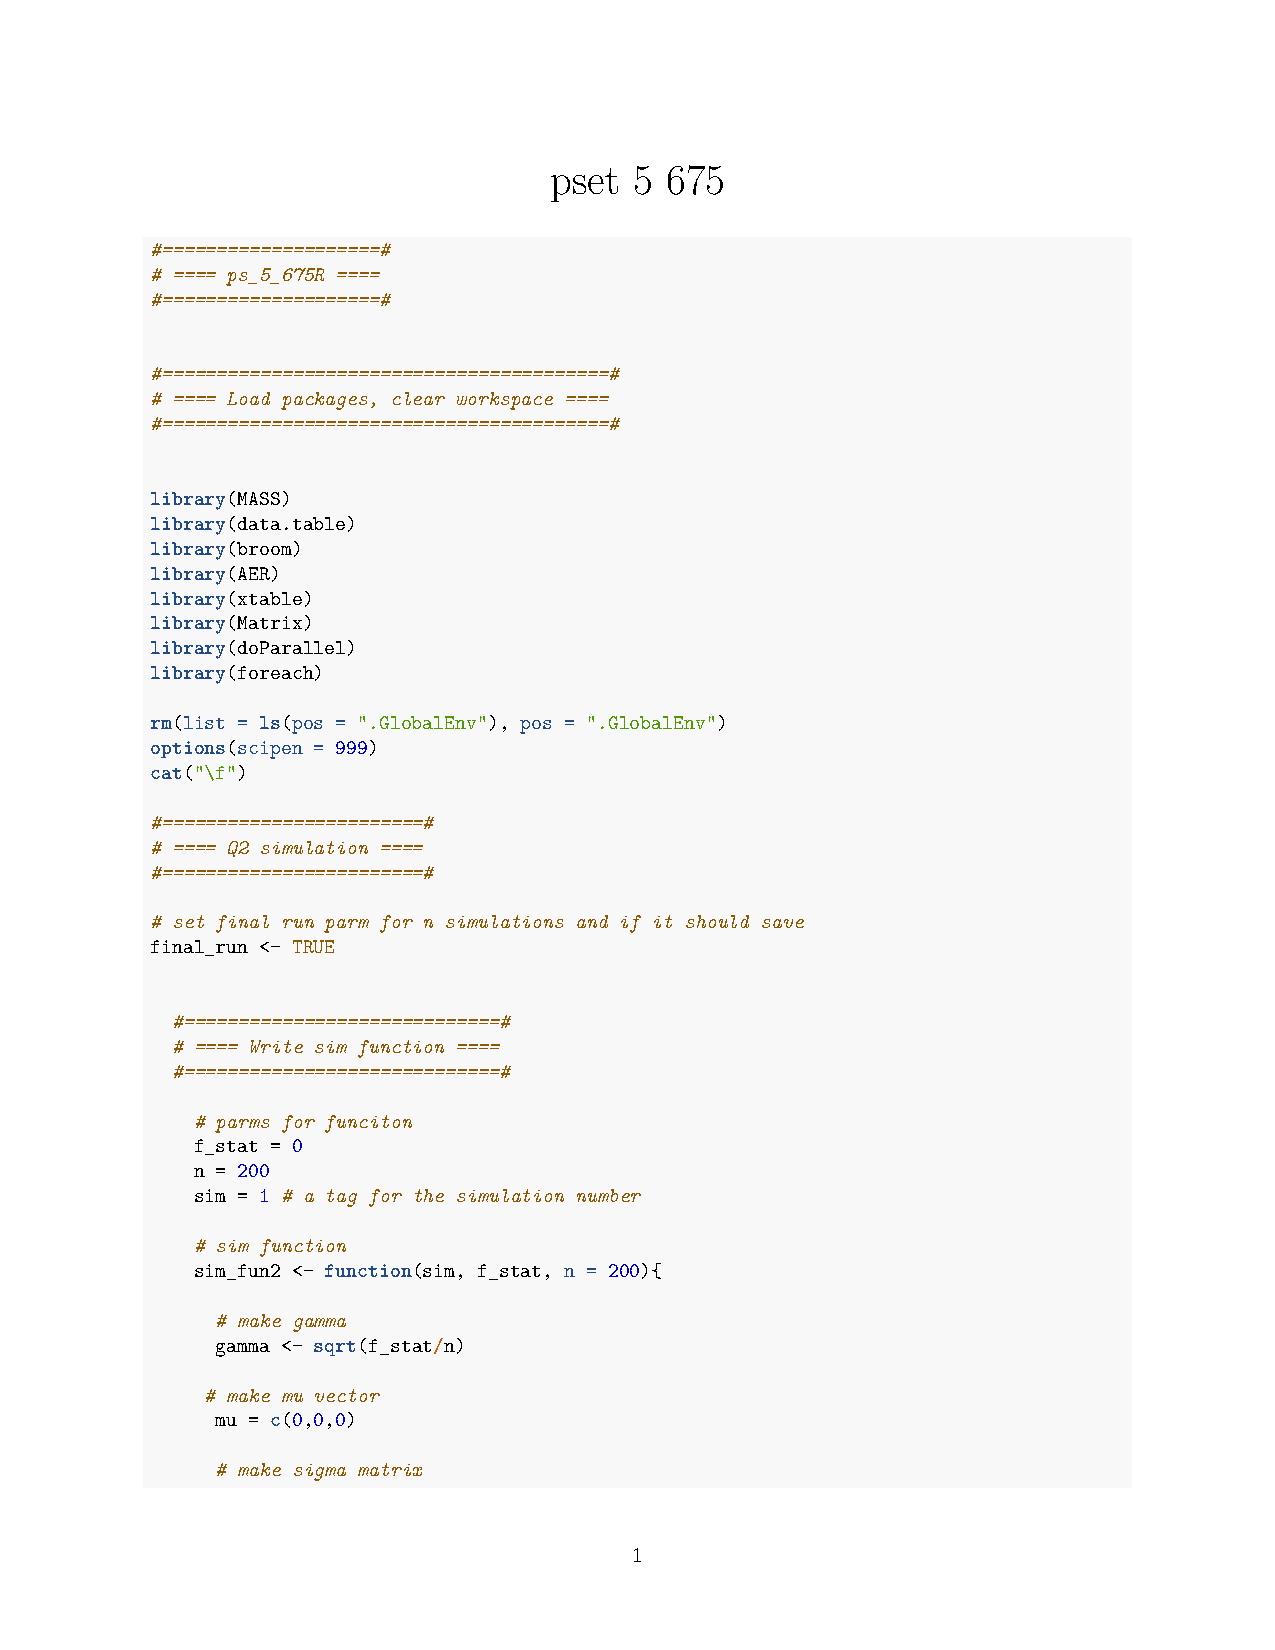
\includepdf[page=-]{assignment_5_r_code_pdf}

\subsection{STATA Code}
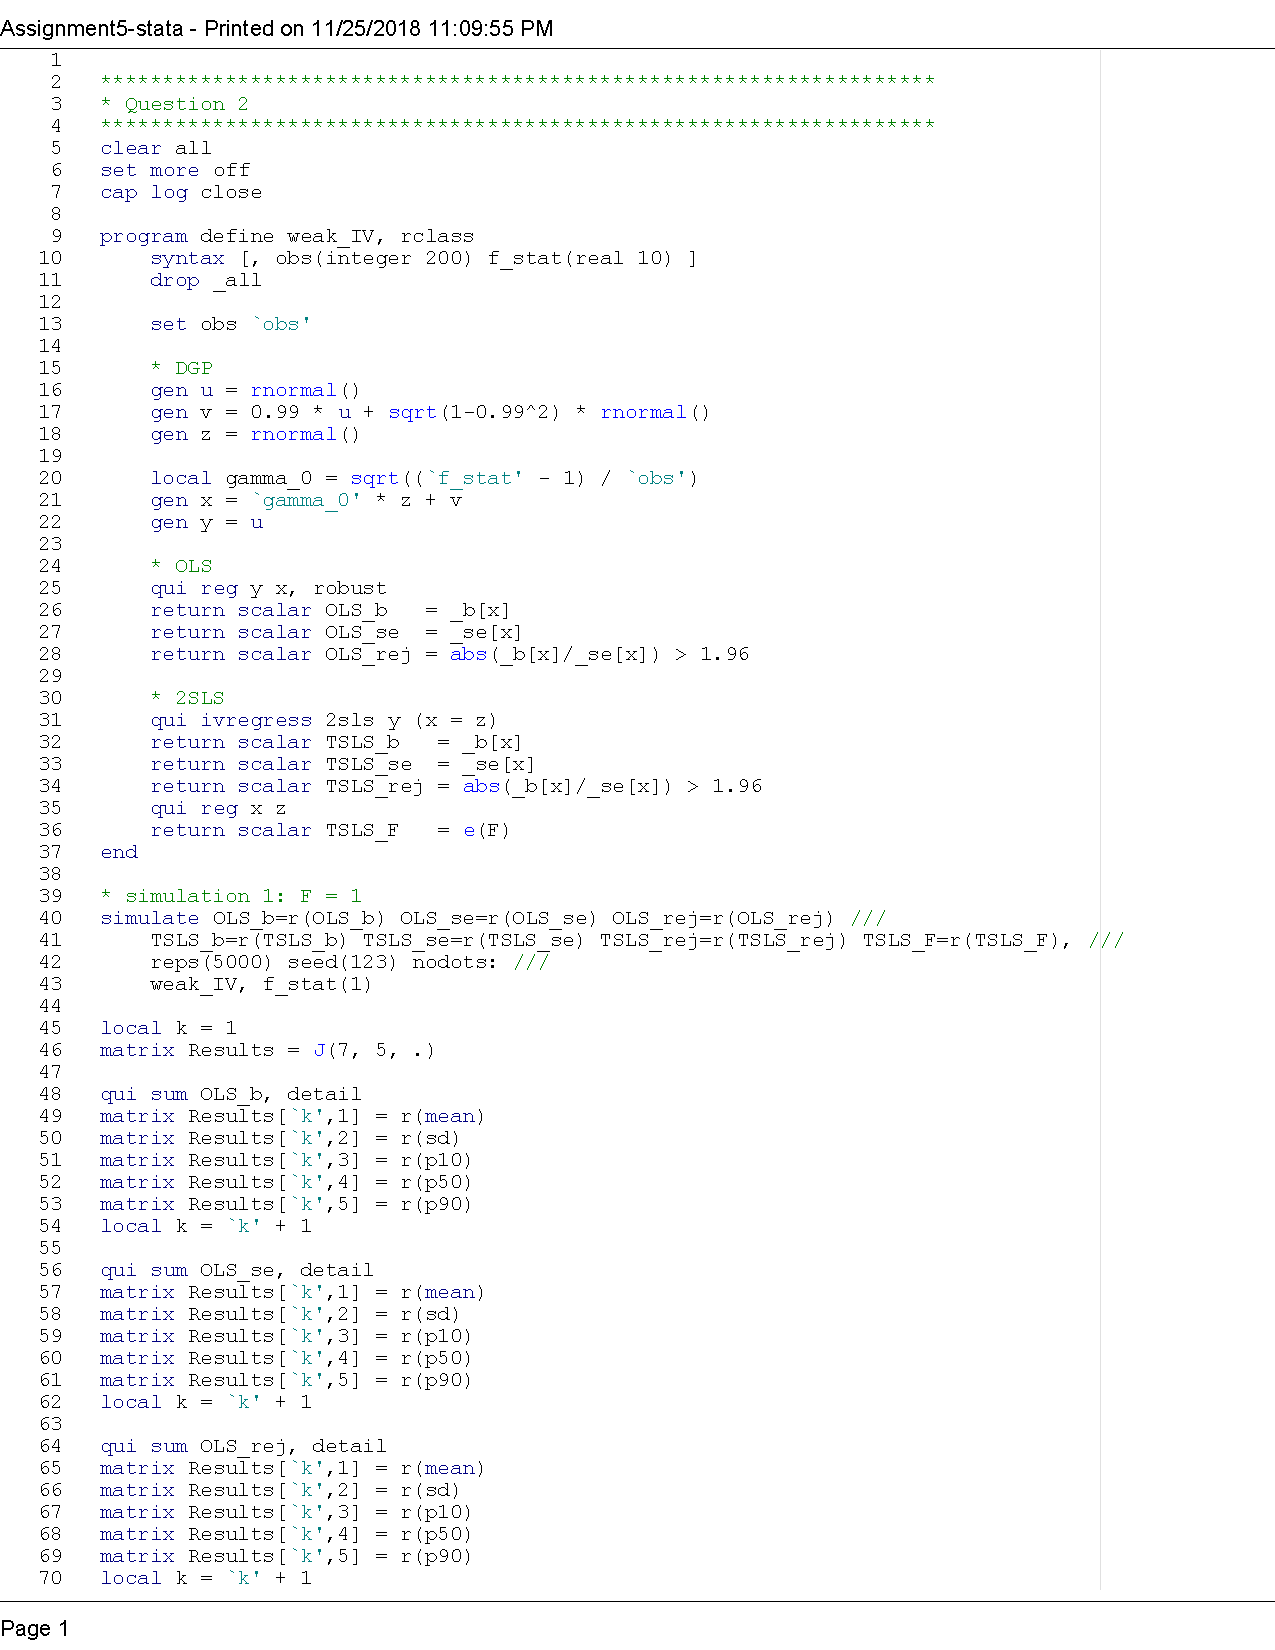
\includepdf[page=-]{assignment_5_stata_code_pdf}

%------------------------------------------------
% end doc
%------------------------------------------------
\end{document}
